
\documentclass[12pt]{article}
\usepackage{fullpage,amsmath,amssymb,graphicx}

\usepackage{setspace}
\spacing{1}

\usepackage{textpos}
\usepackage{tikz}
\usepackage{pgf}
\usepackage{amssymb}
\usepackage{enumerate}
\usepackage{xcolor}
\usepackage{graphicx}
\usepackage{subcaption}
\usepackage{tabularx}
\usepackage{colortbl}
\usepackage{multicol}
\usepackage{longtable}
\usepackage{hyperref}
\usepackage{comment}
\usepackage{listings}



\definecolor{encabezado}{rgb}{0.74, 0.83, 0.9}

\begin{document}

\hfill\\
\rule{\textwidth}{1.5pt}

\begin{minipage}[t]{85mm}
  \begin{tabular}{l}
    \textbf{\large Instituto Tecnológico de Costa Rica} \\  
    \textbf{Escuela de Ingeniería Electrónica} \\
    \textbf{Trabajo Final de Graduación} \\
    \textbf{Proyecto:} Método basado en aprendizaje reforzado \\para el control automático de una planta no lineal. \\
    \textbf{Estudiante:} Oscar Andrés Rojas Fonseca \hspace{3cm}\rule{4.5cm}{1.5pt}\\
    I Semestre 2024 \hspace{8.5cm}\textbf{Firma del asesor}
  \end{tabular}
\end{minipage}
\hfill\\
\rule{\textwidth}{1.5pt}


\section*{Bitácora de trabajo}

%\begin{table}[h]
\begin{minipage}[h]{\textwidth}
	\centering
	\begin{tabularx}{\textwidth}{|p{2cm}|X|X|p{2cm}|} 
		\hline
		\rowcolor{encabezado}
		\textbf{Fecha} & 
		\textbf{Actividad} & 
		\textbf{Anotaciones} & 
		\textbf{Horas dedicadas} \\ \hline
		% ***************************************************************
	 	24/04/2024 & 
	 	$\mathbf{1}.$ Reunión de seguimiento con el asesor del proyecto. & 
	 	$a)$ Revisión de avance y errores de forma. \newline
	 	$b)$ bbbb. \newline & 
	 	2 horas \\
		% ***************************************************************
		26/04/2024 & 
	 	$\mathbf{3}.$ Pruebas de mejora en la función $get\_action()$ del método $PPO$. &
	 	$a)$ ADADADA. \newline & 
	 	4 horas \\
		% ***************************************************************

	 	\hline
	\end{tabularx}
\end{minipage}	 	
	 	
	 	% ***************************************************************
\hfill\\
\begin{minipage}[h]{\textwidth}
	\centering
	\begin{tabularx}{\textwidth}{|p{2cm}|X|X|p{2cm}|} 
		\hline		
		
	 	% ***************************************************************
	 	27/04/2024 & 
	 	$\mathbf{5}.$ Prueba del monetaje del método $DQN$ discretizado para el control del env $PAHM$. &
	 	$a)$ ADADAD \newline & 
	 	4 horas \\
	 	% ***************************************************************
	 	28/04/2024 & 
	 	$\mathbf{6}.$ HFGHDFGHgh. &
	 	$a)$ GGGGGGGG. \newline
	 	$b)$ VVVVVVVVVV. \newline & 
	 	6 horas \\
	 	% ***************************************************************
	 	29/04/2024 & 
	 	$\mathbf{6}.$ Pruebas de entrenamiento del modelo $PPO$ del $PAHM$. &
	 	$a)$ Probando métodos de distribucion normal y otros. \newline
	 	$b)$ ASDASD. \newline & 
	 	6 horas \\
	 	% ***************************************************************
	 	30/04/2024 & 
	 	$\mathbf{6}.$ AAAAAAAAAA. &
	 	$a)$ RRRRRR. \newline
	 	$b)$ WWWWWWWWW. \newline & 
	 	6 horas \\
	 	% ***************************************************************
	 	
	 	\hline
		\multicolumn{3}{|r|}{Total de horas de trabajo:} & 64 horas \\ 
	 	\hline                 
	\end{tabularx}
\end{minipage}





% *****************************************************************************
% *****************************************************************************
% *****************************************************************************

\section*{Contenidos de actividades}

AAA \cite{Airdaldi2023}

%\begin{figure}[h!]
%	\centering
%	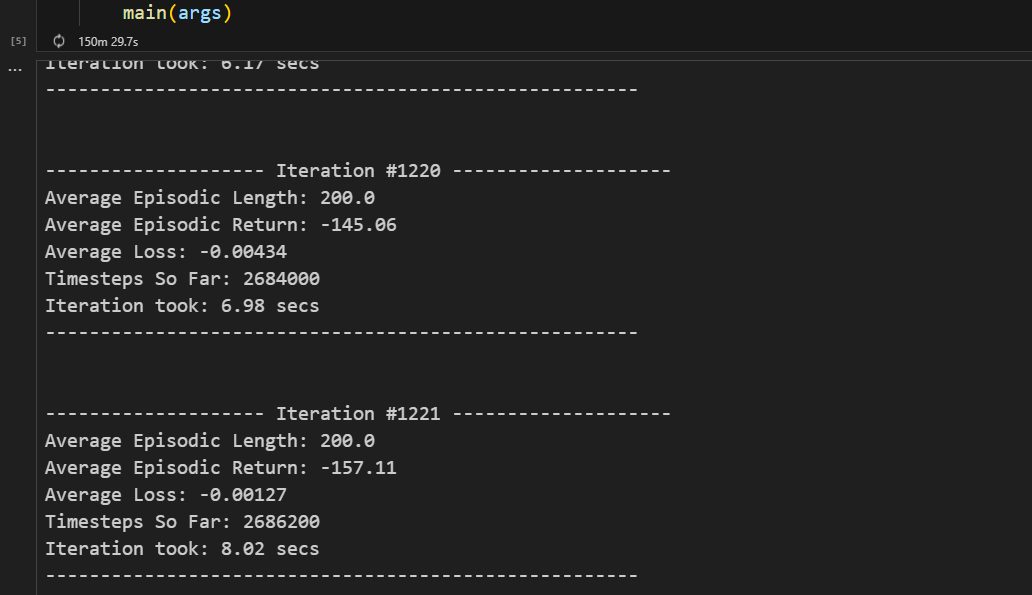
\includegraphics[scale=0.45]{Fig/Captura_PPO_200Me.png}
%	\caption{Proceso de entrenamiento del modelo para $PendulumPPO$ con $200M$ de episodios.}
%	\label{fig:PendPPOv1}
%\end{figure}	


\newpage

\section*{Referencias}
\renewcommand\refname{}
\bibliographystyle{IEEEtran}
\bibliography{references}





\end{document}
